\chapter{Finding Optimal Hyperparameters for the Cleaning Algorithms}%
\label{ch:finding-hyperparams}

This work aims to find optimal hyperparameters for the cleaning algorithms used in \ctapipe{}.
Optimizing the cleaning step of the \dlo{} data level in \autoref{sec:data-levels} can most certainly lead to a better
reconstruction of the events in a dataset. Therefore, a tweaking of the available parameters of each
cleaner is necessary. In this chapter, I will first introduce the cleaning algorithms and their parameters
in \autoref{sec:cleaning-algorithms} and then describe the procedure to find optimal hyperparameters
in \autoref{sec:hyperparameters}.
\vspace{-0.5cm}
\section{Cleaning Algorithms}%
\label{sec:cleaning-algorithms}
\vspace{-0.5cm}
\subsection*{\texttt{TailcutsImageCleaner}}%
\vspace{-0.2cm}
The version of \ctapipe{} used features four cleaning algorithms, two of which are time-based.
The \tailcuts{} algorithm is the most basic algorithm of the four and serves as a good
starting point for the development of new cleaning algorithms. Its first step is to select all
pixels that are above a certain threshold, the core threshold \(Q_c\) (also called picture threshold in \ctapipe{}). These
pixels are the core part of the signal and are the brightest. The \tailcuts{} algorithm
then selects all pixels that are above the boundary threshold \(Q_b\) and are neighboring
the core pixels. A visualization of the algorithm is shown in \autoref{fig:tailcuts_clean} for the
default values of the algorithm.

\begin{figure}
    \centering
    % \begin{subfigure}[t]{0.33\textwidth}
    %     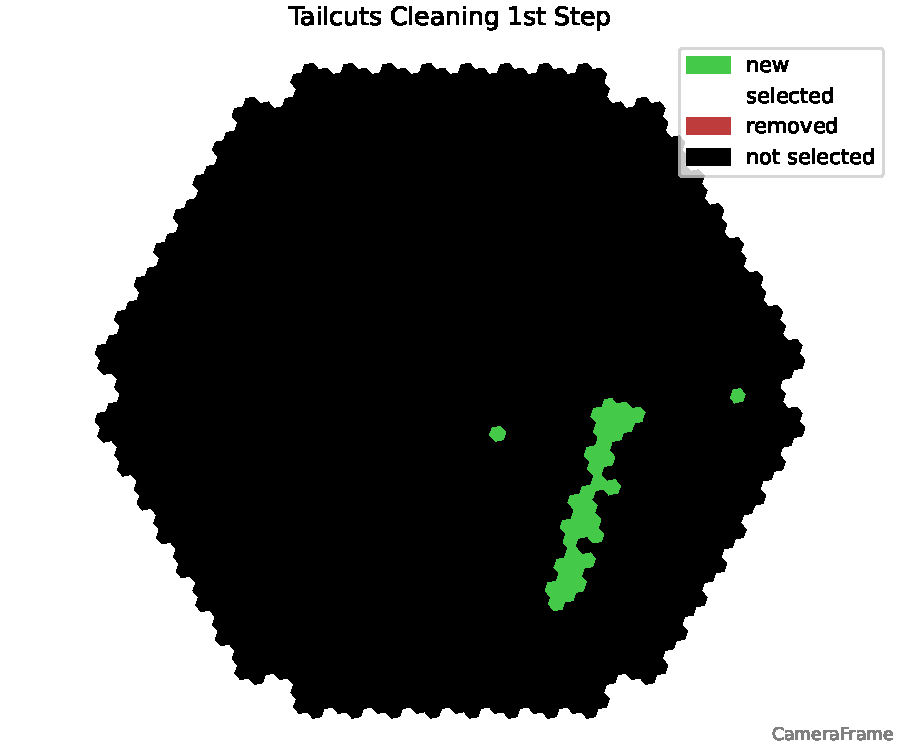
\includegraphics[width=\textwidth]{plots/cleaner_steps/tail_1.pdf}
    % \end{subfigure}
    % \begin{subfigure}[t]{0.33\textwidth}
    %     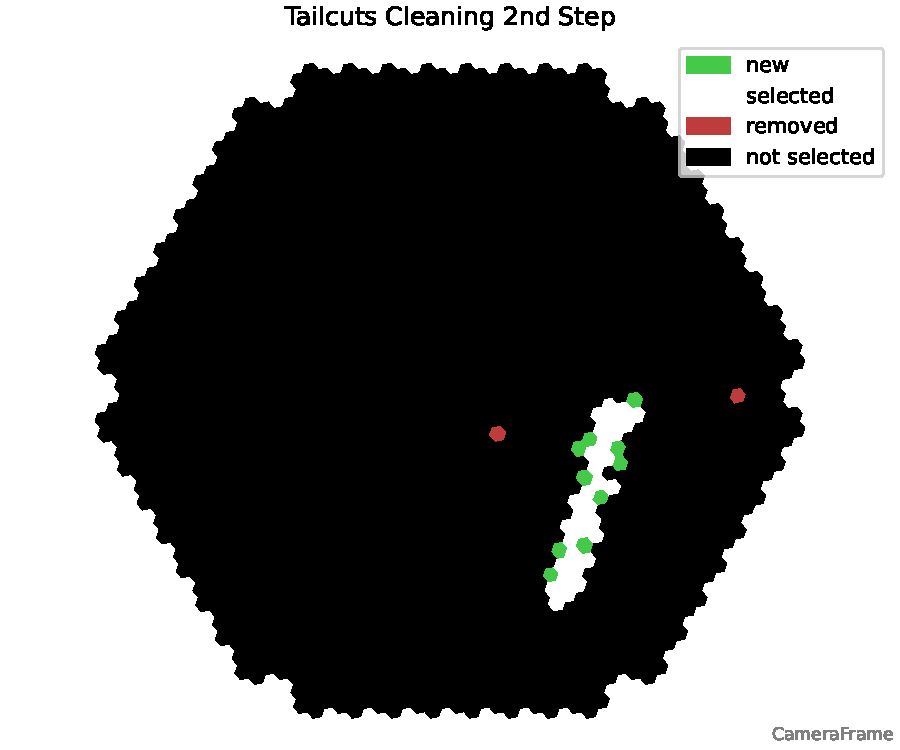
\includegraphics[width=\textwidth]{plots/cleaner_steps/tail_2.pdf}
    % \end{subfigure}
    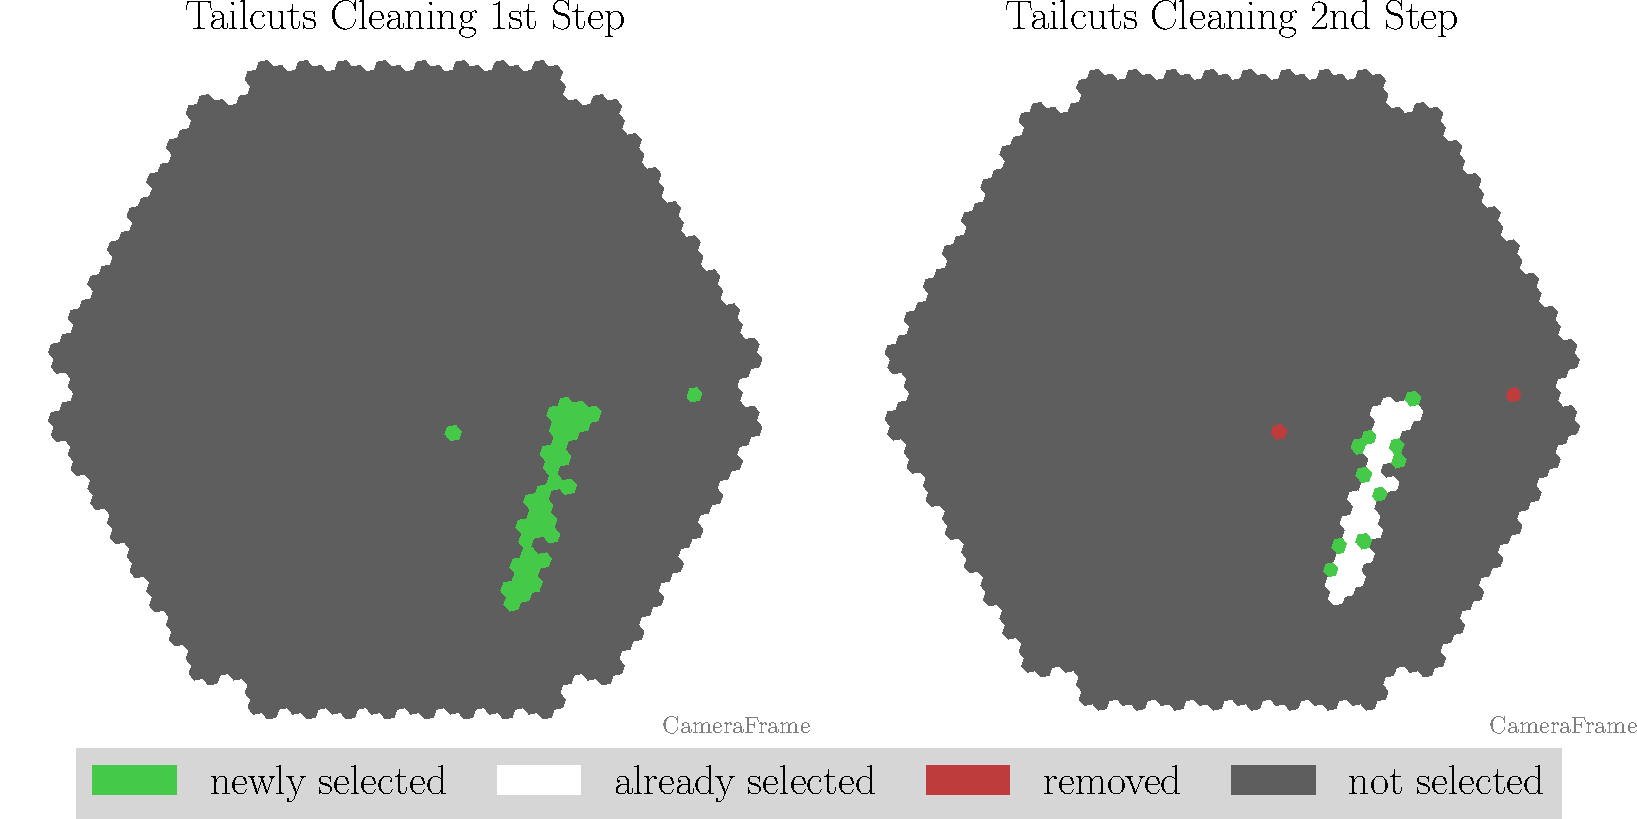
\includegraphics[height=4cm]{plots/cleaner_steps/tailcuts.pdf}
    \caption{Visualization of the \tailcuts{} algorithm for a \gls{mst} NectarCam image. First, all
    pixels above the core threshold are selected. Then, all pixels neighboring the core
    pixels that are above the boundary threshold are selected.}%
    \label{fig:tailcuts_clean}
\end{figure}

\subsection*{\texttt{MARSImageCleaner}}%
\vspace{-0.2cm}
The \mars{} algorithm~\cite{mars} is very much based on the \tailcuts{}
algorithm and features an additional step, in that it also selects all neighbors of a neighbor of a
core pixel, if they are above the boundary threshold. The three steps for the \mars{} algorithm
are shown in \autoref{fig:mars_cleaning} for its default values.
\begin{figure}[!htbp]
    \centering
    % \begin{subfigure}[t]{0.32\textwidth}
    %     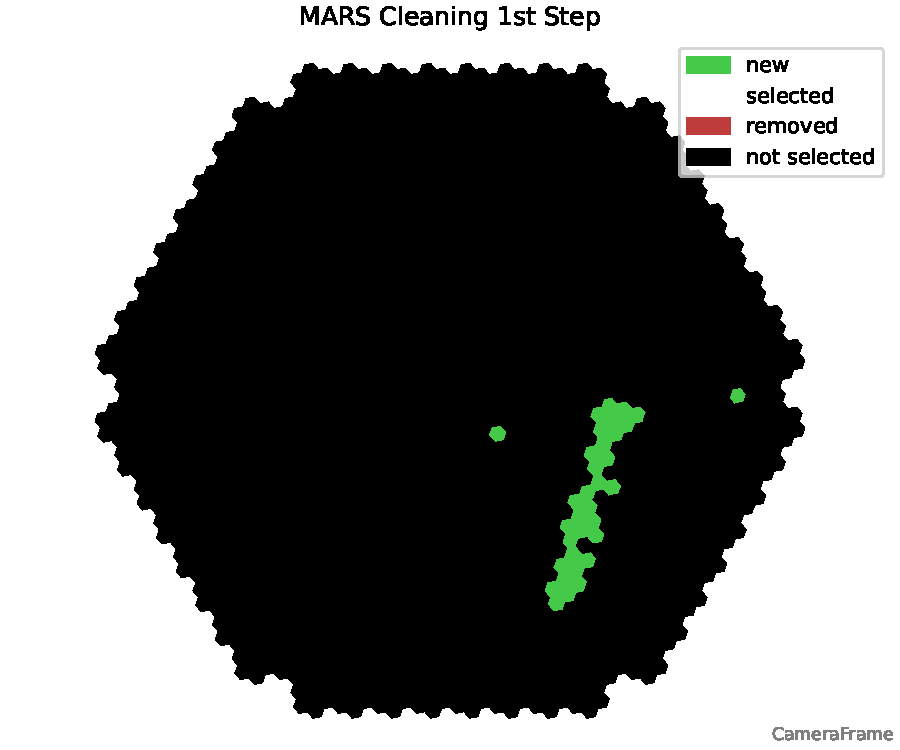
\includegraphics[width=\textwidth]{plots/cleaner_steps/mars_1.pdf}
    % \end{subfigure}
    % \hfill
    % \begin{subfigure}[t]{0.32\textwidth}
    %     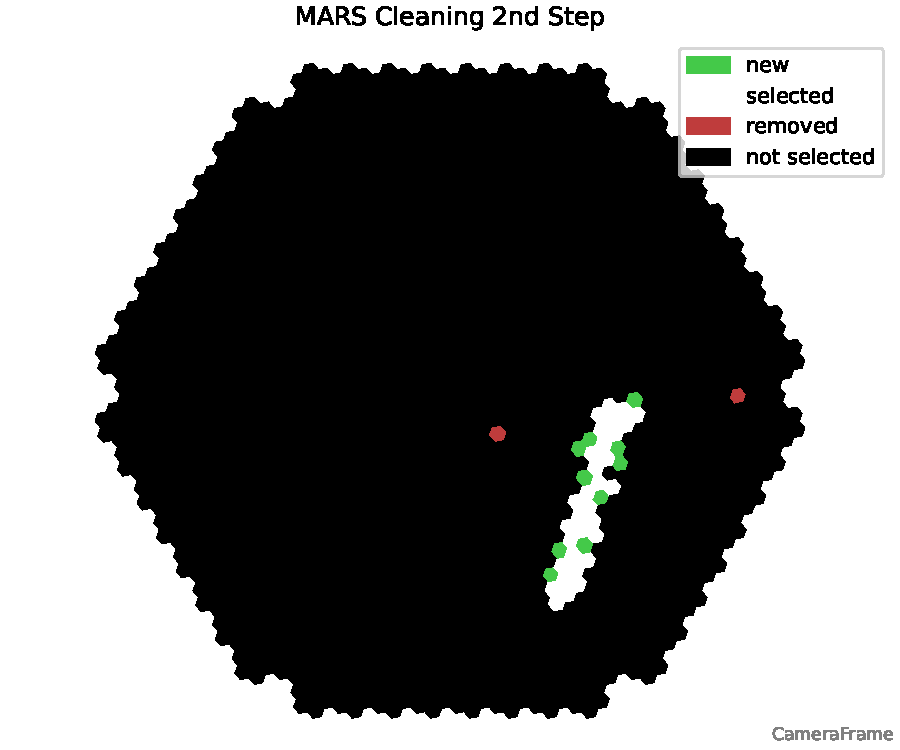
\includegraphics[width=\textwidth]{plots/cleaner_steps/mars_2.pdf}
    % \end{subfigure}
    % \hfill
    % \begin{subfigure}[t]{0.32\textwidth}
    %     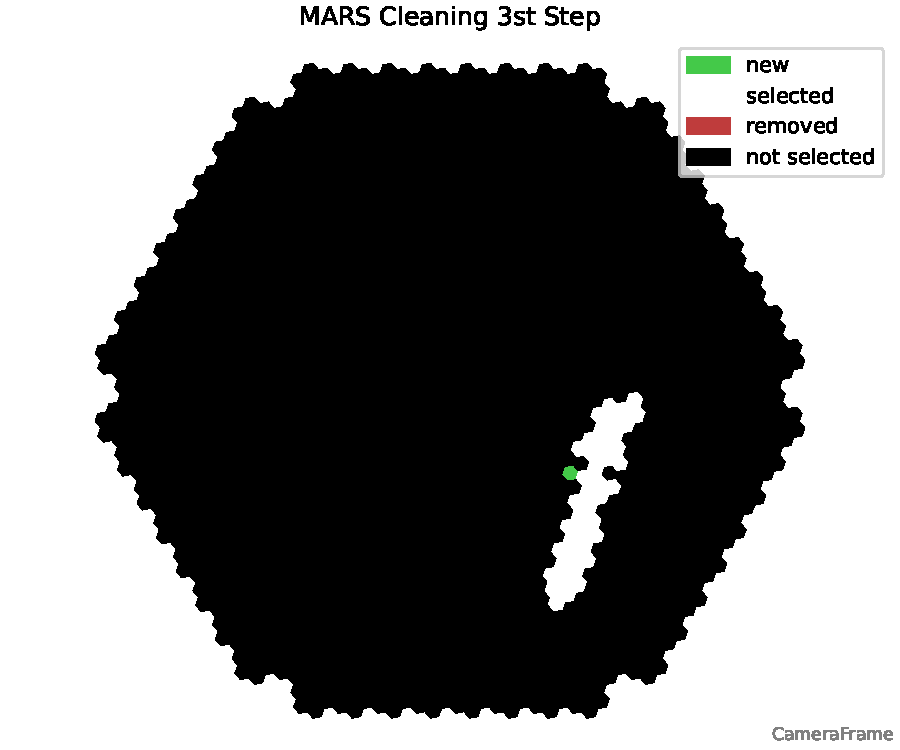
\includegraphics[width=\textwidth]{plots/cleaner_steps/mars_3.pdf}
    % \end{subfigure}
    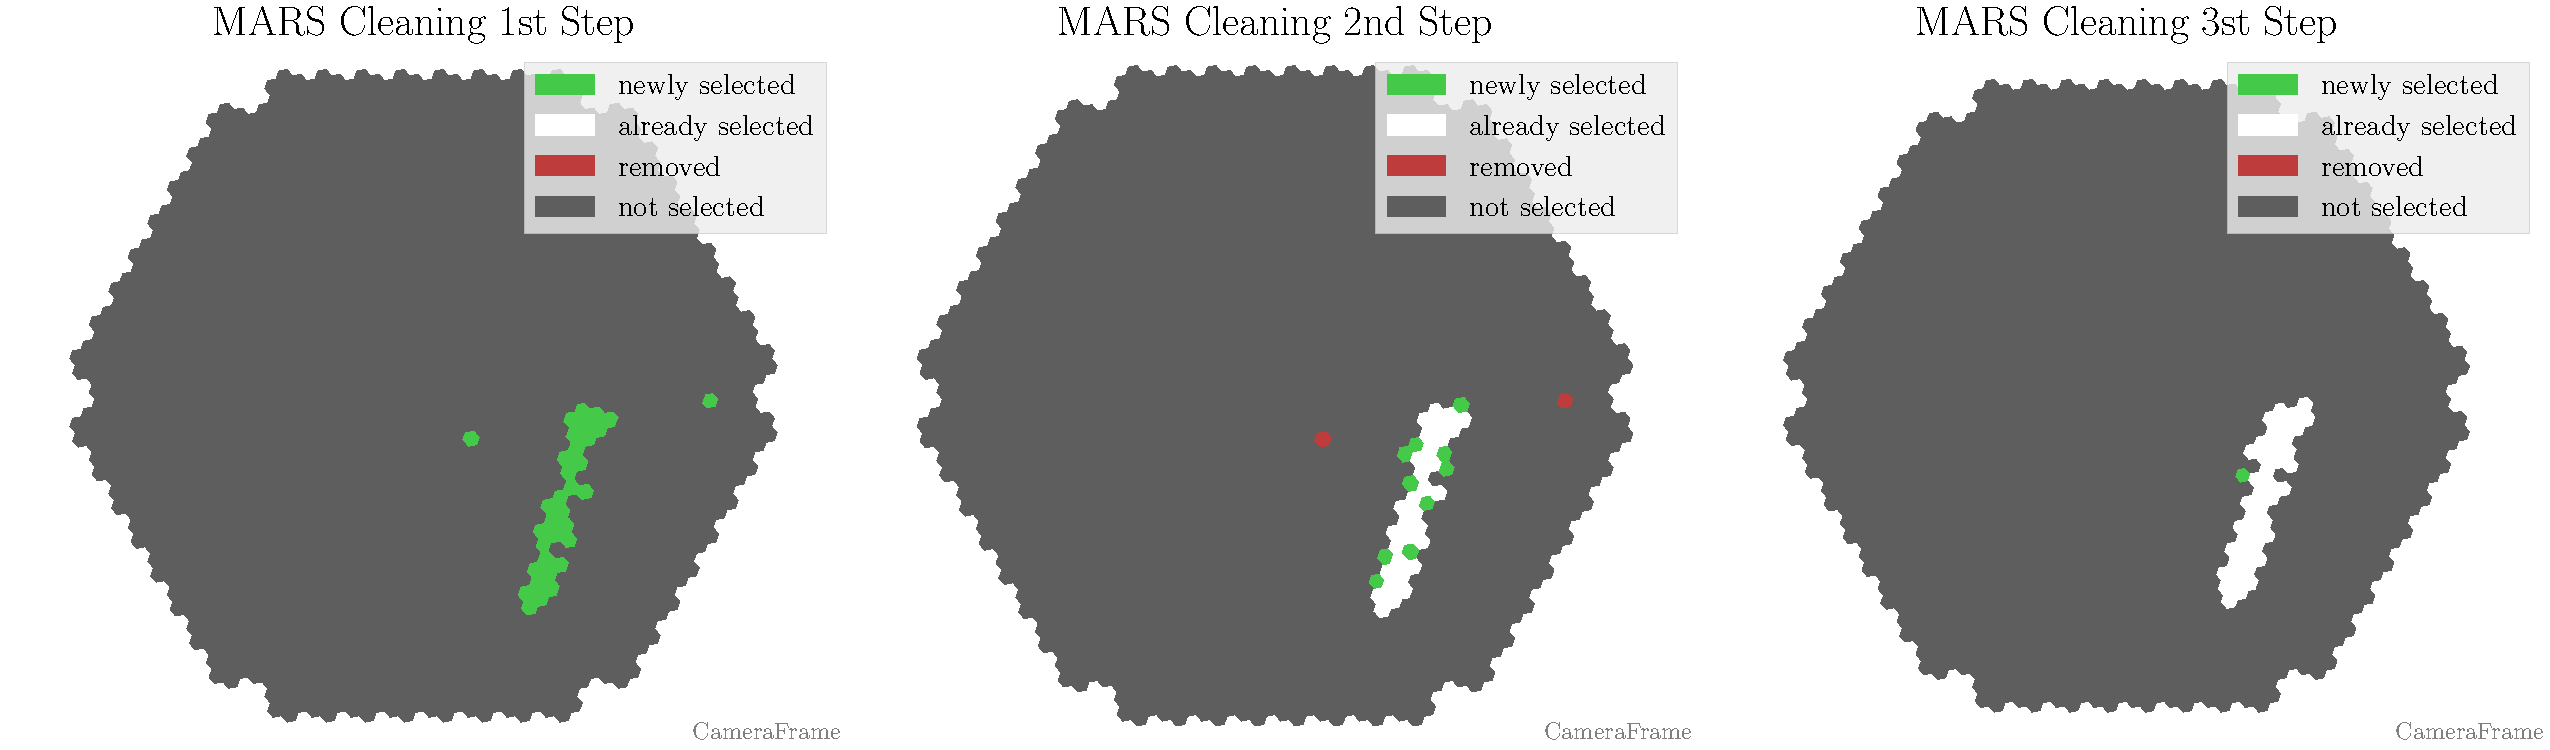
\includegraphics[height=4cm]{plots/cleaner_steps/mars.pdf}
    \caption{Visualization of the \mars{} algorithm for a \gls{mst} NectarCam image. The first two
    steps are identical to the \tailcuts{} algorithm. The third step selects all neighbors of a neighbor of a
    core pixel if they are above the boundary threshold \(Q_b\).}%
    \label{fig:mars_cleaning}
\end{figure}
\begin{figure}[!htbp]
    \centering
    % \begin{subfigure}[t]{0.32\textwidth}
    %     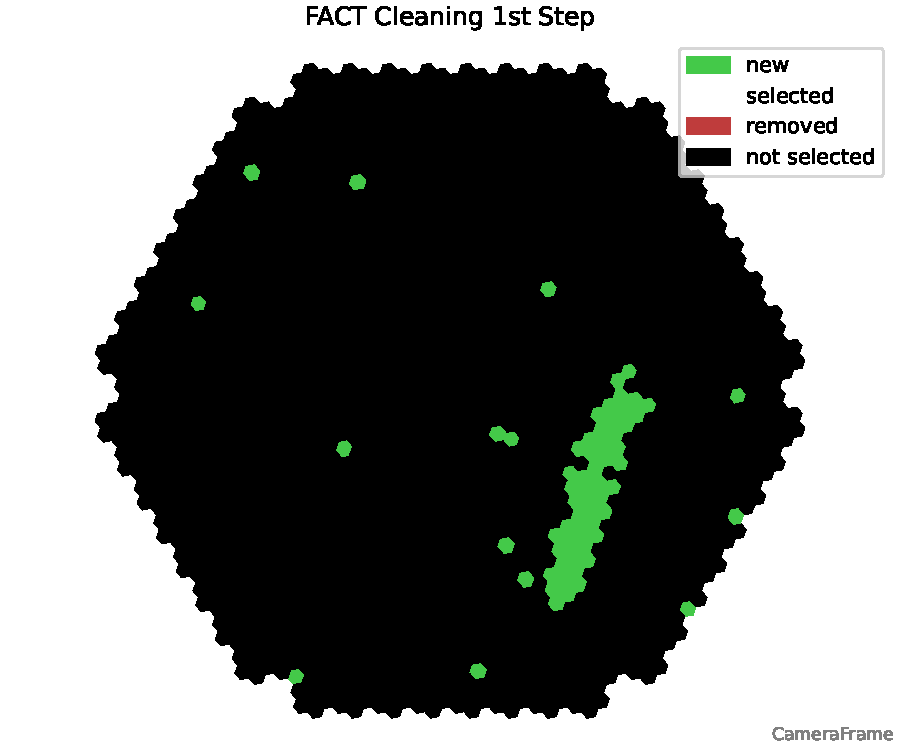
\includegraphics[width=\textwidth]{plots/cleaner_steps/fact_1.pdf}
    % \end{subfigure}
    % \hfill
    % \begin{subfigure}[t]{0.32\textwidth}
    %     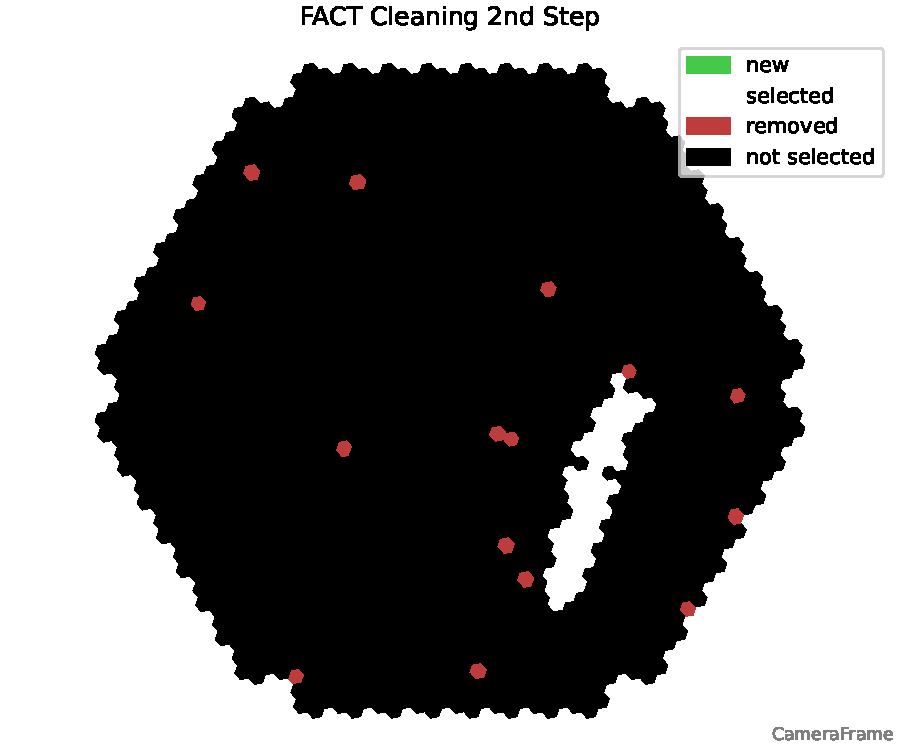
\includegraphics[width=\textwidth]{plots/cleaner_steps/fact_2.pdf}
    % \end{subfigure}
    % \hfill
    % \begin{subfigure}[t]{0.32\textwidth}
    %     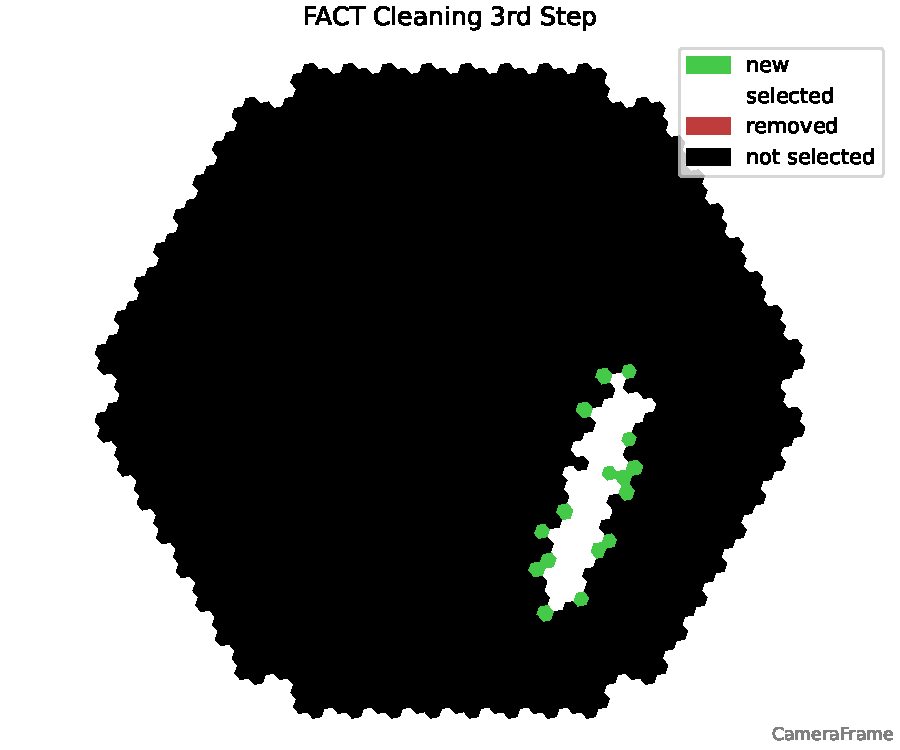
\includegraphics[width=\textwidth]{plots/cleaner_steps/fact_3.pdf}
    % \end{subfigure}
    % \begin{subfigure}[b]{0.32\textwidth}
    %     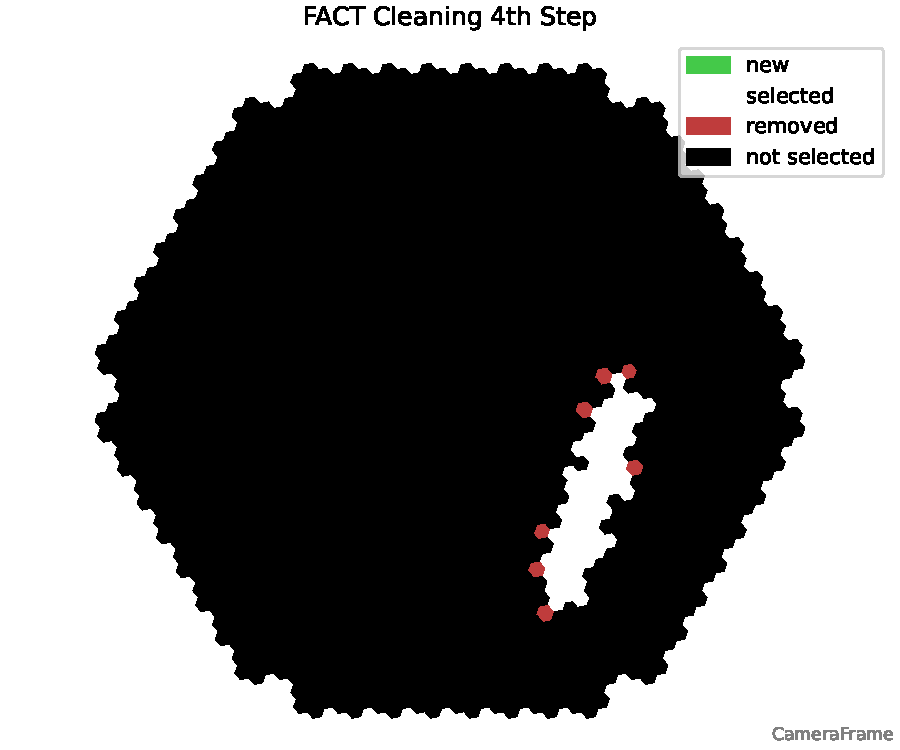
\includegraphics[width=\textwidth]{plots/cleaner_steps/fact_4.pdf}
    % \end{subfigure}
    % \hfill
    % \begin{subfigure}[b]{0.32\textwidth}
    %     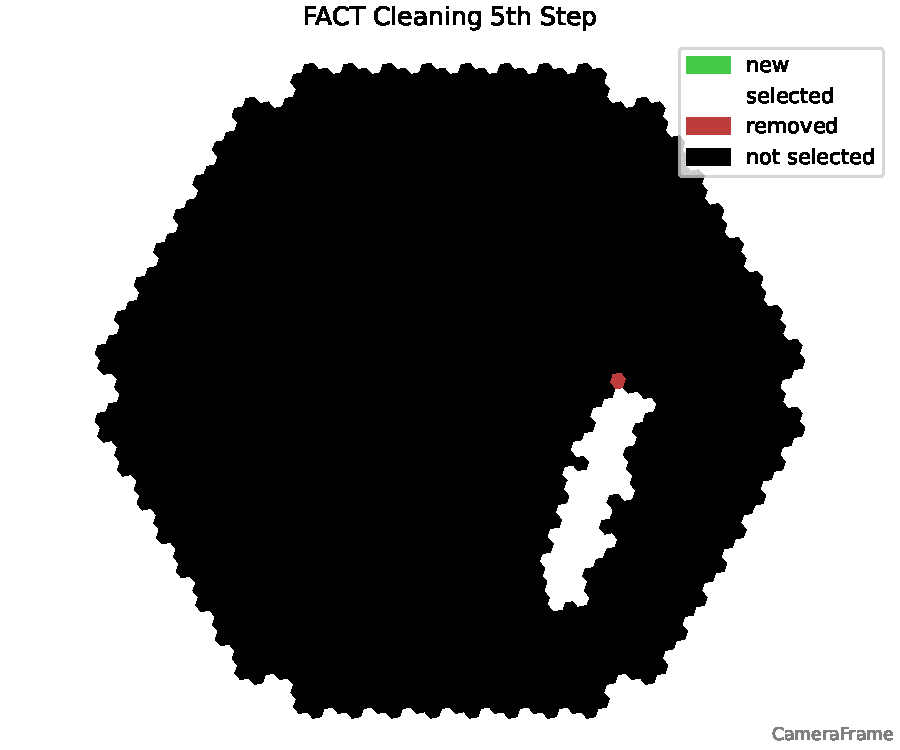
\includegraphics[width=\textwidth]{plots/cleaner_steps/fact_5.pdf}
    % \end{subfigure}
    % \hfill
    % \begin{subfigure}[b]{0.32\textwidth}
    %     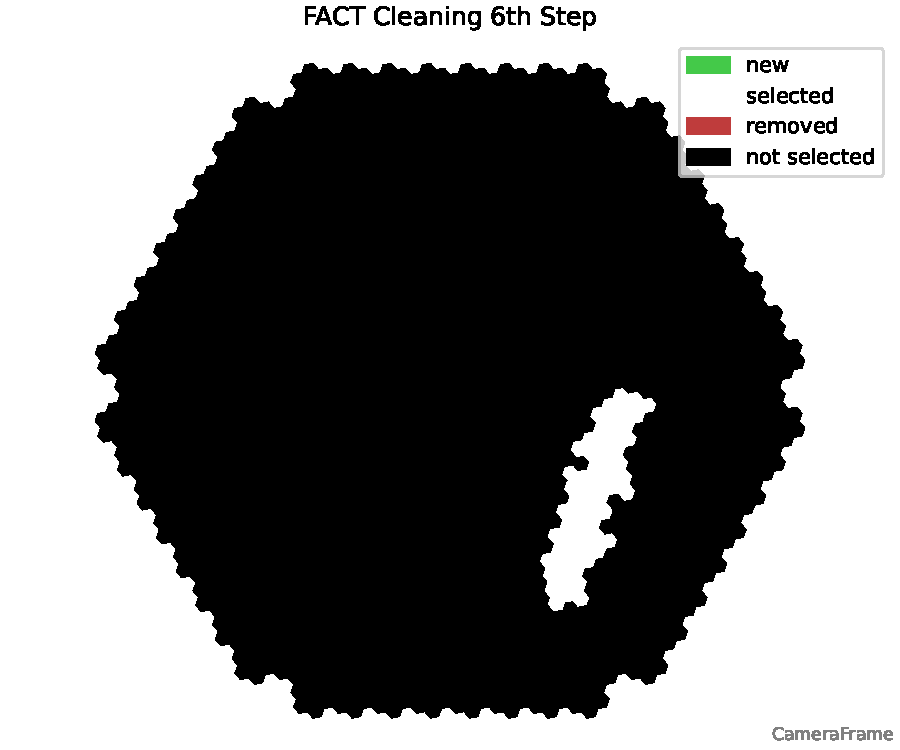
\includegraphics[width=\textwidth]{plots/cleaner_steps/fact_6.pdf}
    % \end{subfigure}
    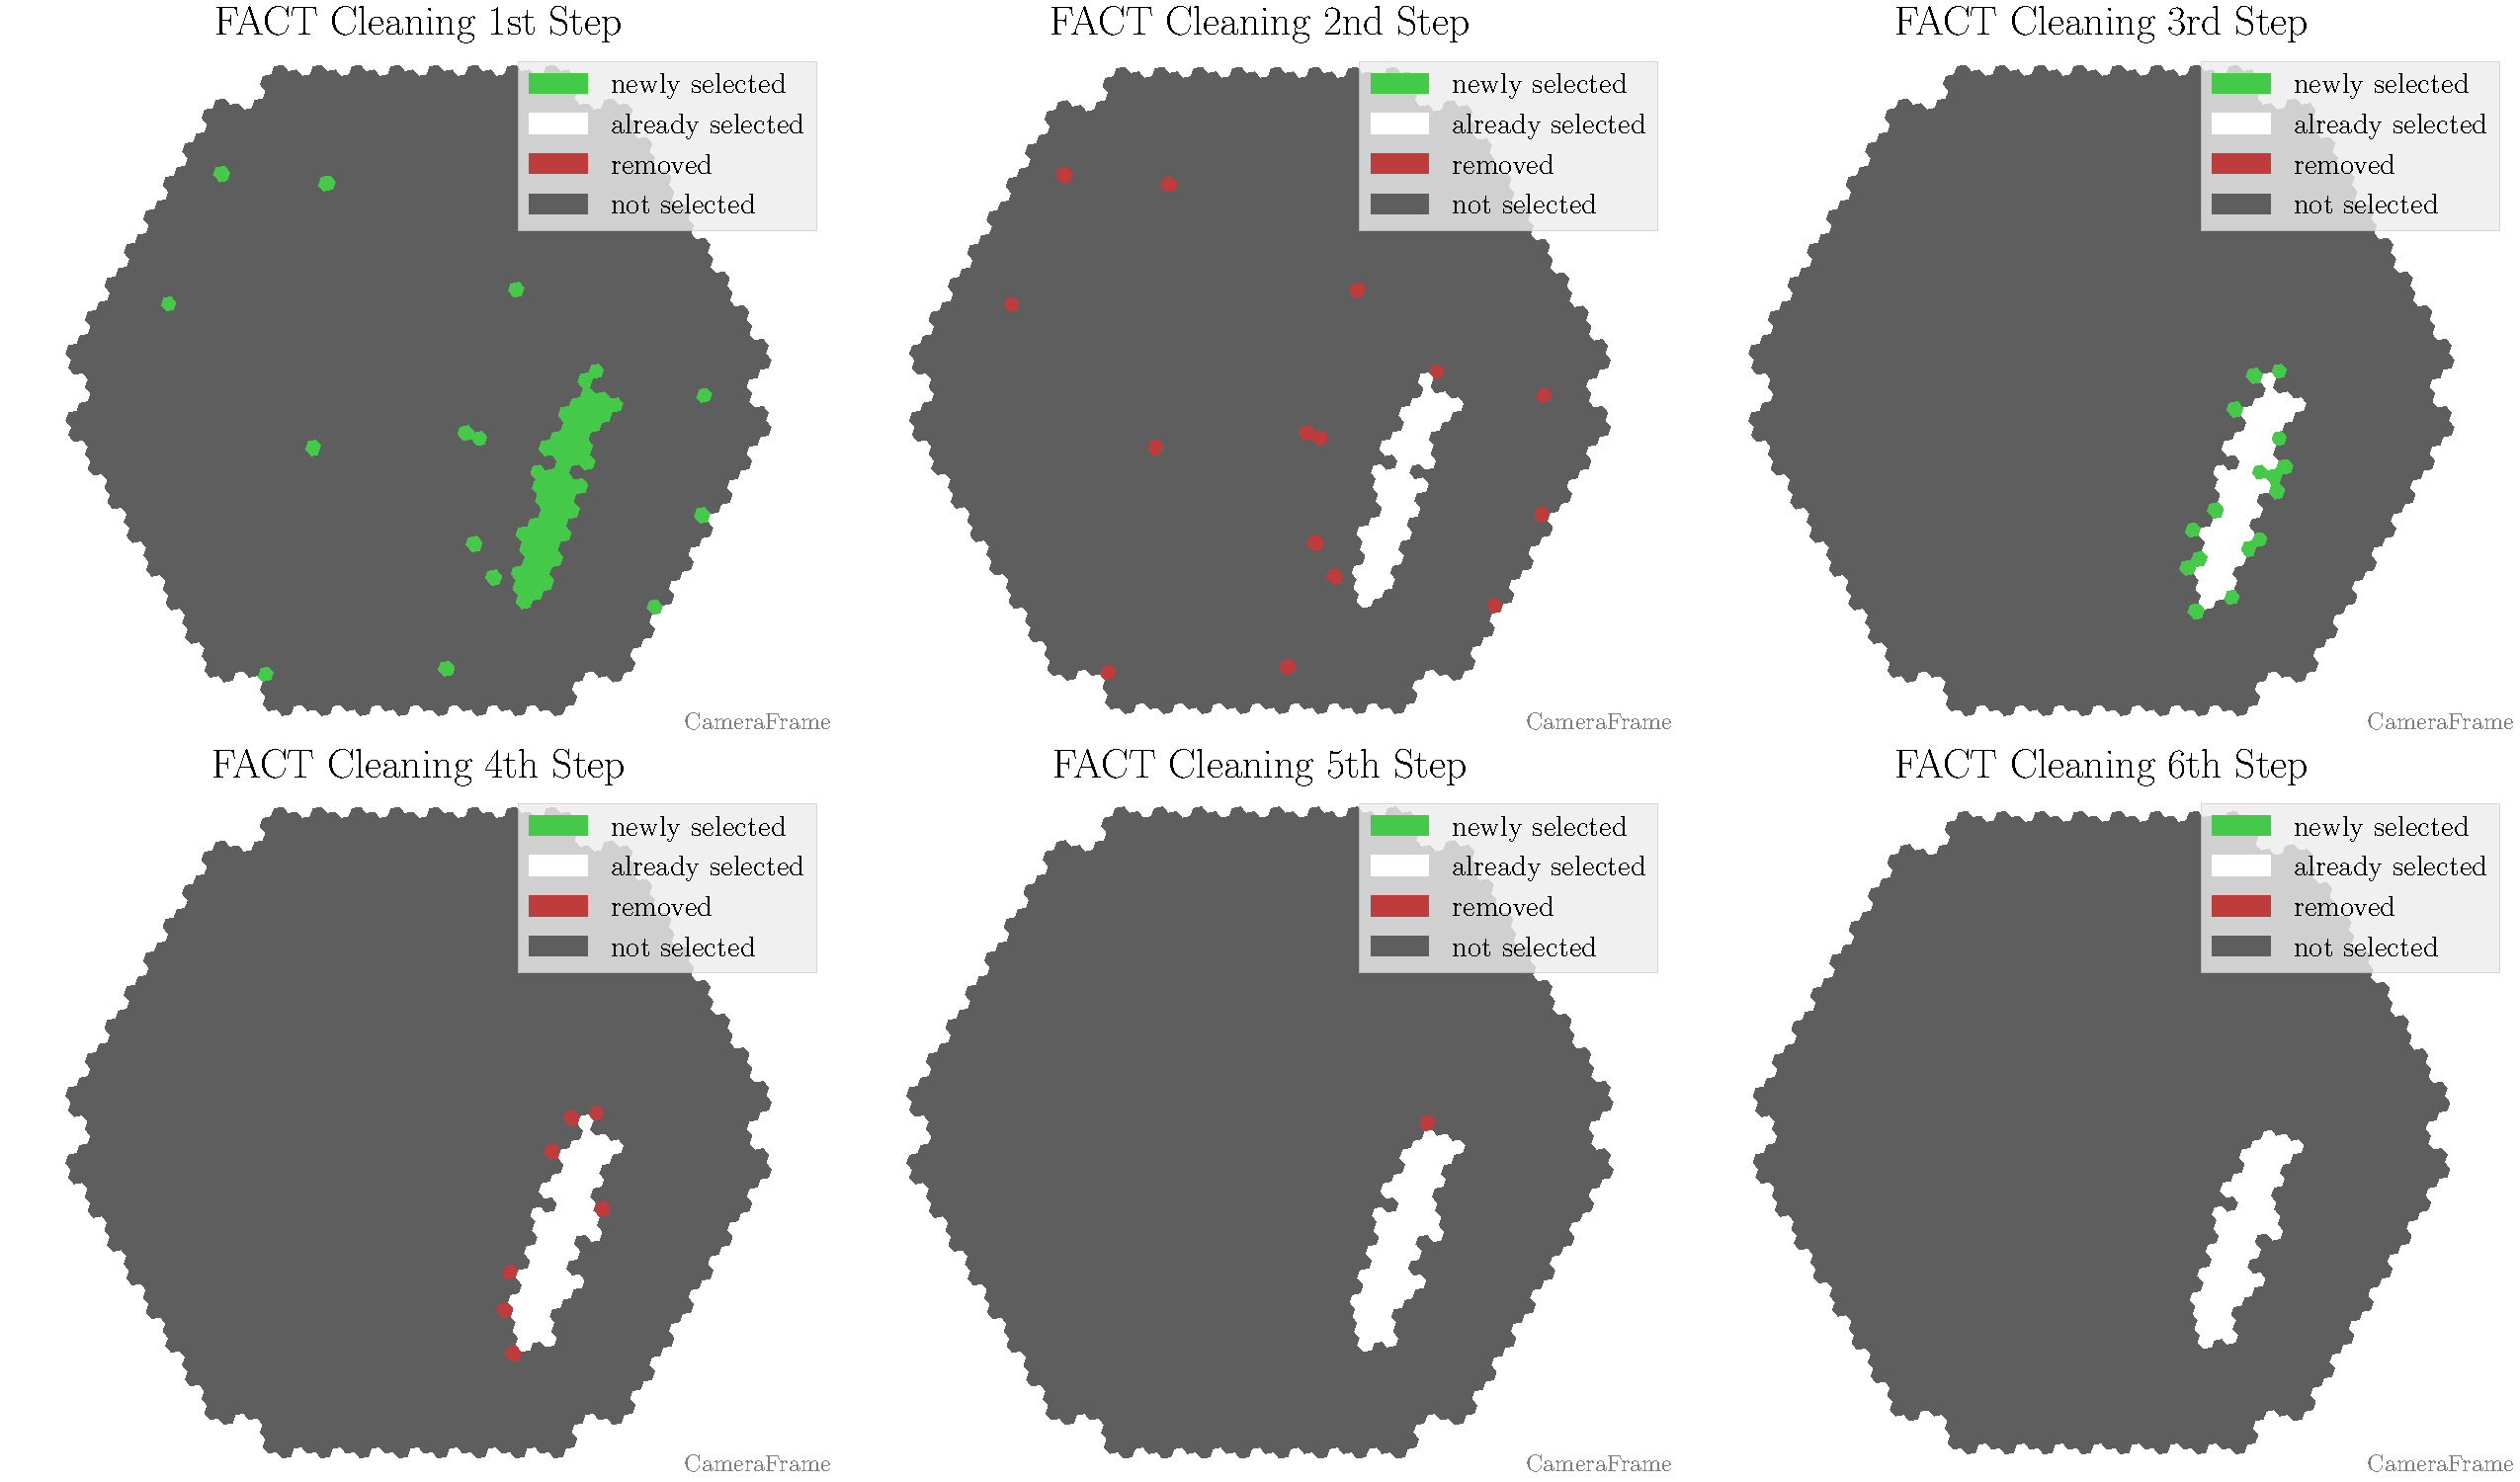
\includegraphics[height=8cm]{plots/cleaner_steps/fact.pdf}
    \caption{Visualization of the \fact{} algorithm for a \gls{mst} NectarCam image. The first
    step selects all pixels above the core threshold \(Q_c\). The second step removes all pixels that have less than
    \(N\) neighbors. The third step selects all pixels neighboring the remaining pixels that are above the
    boundary threshold \(Q_b\). The fourth step removes all pixels that have less than \(N\) neighbors,
    that have arrived within a given timeframe. The fifth and sixth steps are analogous to steps two and four respectively.
    Notice, that---per default in \ctapipe---the values for \(Q_c\) and \(Q_b\) are lower than for the other cleaners
    (see \autoref{tab:hyperparameters}), and hence together with the time limit more individual pixels than in the
    other cleaning algorithms are selected in the first step.}%
    \label{fig:fact_cleaning}
\end{figure}
\subsection*{\texttt{FactImageCleaner}}%
\vspace{-0.5cm}
The \fact{} algorithm~\cite{temme_thesis, temme_diploma} is a time-based cleaning algorithm that first selects all pixels that are above
\(Q_c\). Then, all pixels that have less than \(N\) neighbors are removed.
% Per default, the algorithm looks for a minimum of at least \(\num{2}\) neighbors.
For the third step, all pixels neighboring
the remaining pixels that are above \(Q_b\) are selected. After that, all
pixels that have less than \(N\) neighbors and that have arrived within a given timeframe are removed.
% This timeframe is set to \(\SI{5}{\nano\second}\) by default.
Again, all pixels with less than \(N\) neighbors are removed. The last step once again removes pixels with less than
\(N\) neighbors, arriving within the given time limit. The visualization of the algorithm is shown in
\autoref{fig:fact_cleaning} for the default values of the algorithm.
\vspace{-0.75cm}
\subsection*{\texttt{TimeConstrainedImageCleaner}}%
\vspace{-0.5cm}
The \tcc{} algorithm is another time-based algorithm, coming from the \gls{magic} collaboration~\cite{tcc}.
It first selects all pixels that are above \(Q_c\). Then, all pixels that have
less than \(N\) neighbors are removed. A minimum of \(\num{1}\) neighboring pixel is needed in the default
settings. After that, all core pixels whose arrival times are within a given timeframe of the average arrival time.
% This core time limit \(t_c\) is set to \(\SI{4.5}{\nano\second}\) by default.
As a fourth step, the \tcc{} algorithm finds all pixels above \(Q_b\). Then, all pixels with
less than \(N\) neighbors arriving within a given timeframe are removed.
% This boundary time limit is set to \(\SI{1.5}{\nano\second}\) by default.
The visualization of the algorithm is shown in \autoref{fig:tcc_cleaning} for the default values of the algorithm.
For a better comparison, the resulting cleaned images of each cleaner are shown in \autoref{fig:cleaners_together}
in \hyperref[ap:additional_plots_tables]{appendix~\ref{ap:additional_plots_tables}}.
\begin{figure}
    \centering
    % \begin{subfigure}[t]{0.32\textwidth}
    %     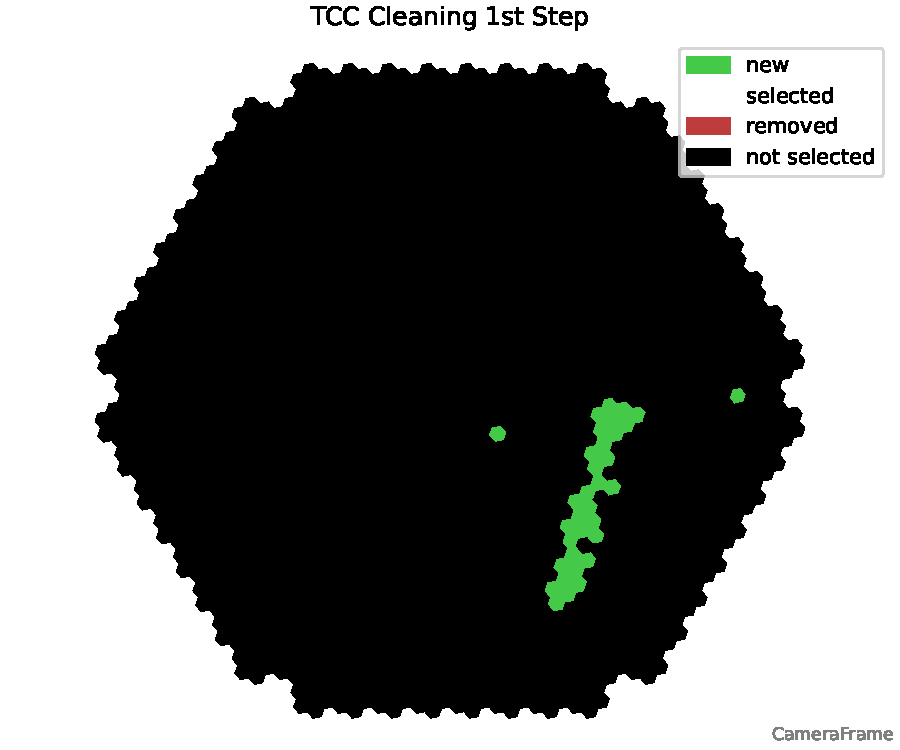
\includegraphics[width=\textwidth]{plots/cleaner_steps/tcc_1.pdf}
    % \end{subfigure}
    % \hfill
    % \begin{subfigure}[t]{0.32\textwidth}
    %     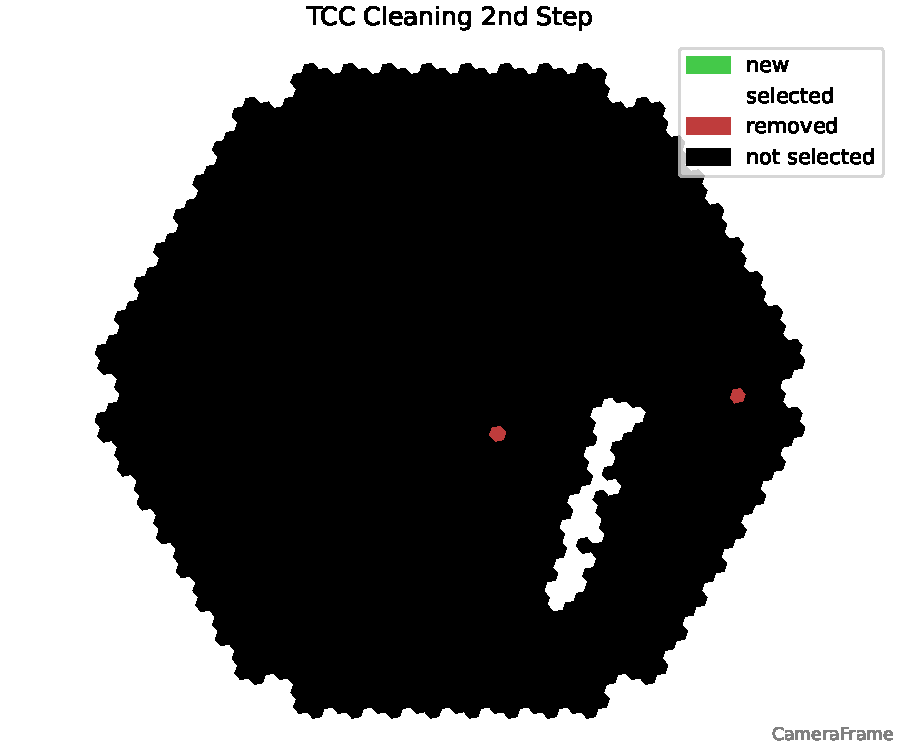
\includegraphics[width=\textwidth]{plots/cleaner_steps/tcc_2.pdf}
    % \end{subfigure}
    % \hfill
    % \begin{subfigure}[t]{0.32\textwidth}
    %     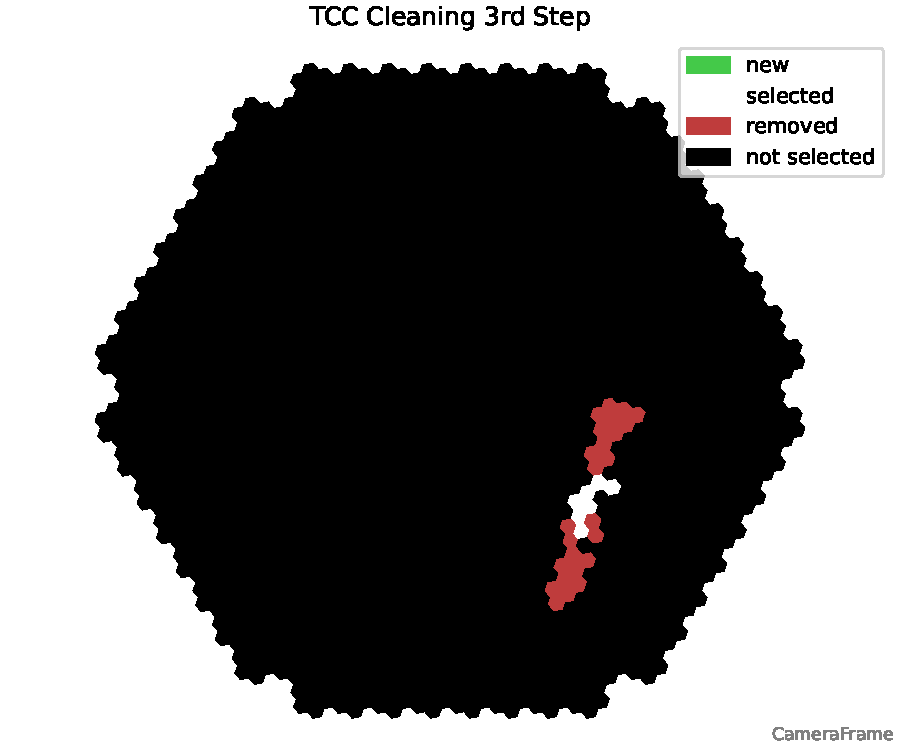
\includegraphics[width=\textwidth]{plots/cleaner_steps/tcc_3.pdf}
    % \end{subfigure}
    % \begin{subfigure}[]{0.32\textwidth}
    %     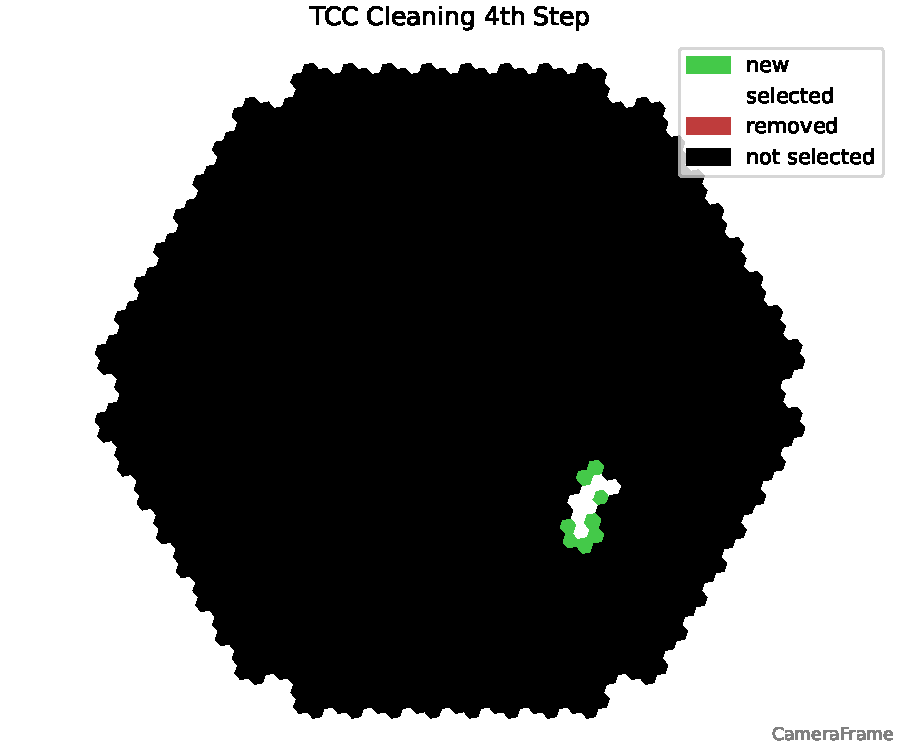
\includegraphics[width=\textwidth]{plots/cleaner_steps/tcc_4.pdf}
    % \end{subfigure}
    % \begin{subfigure}[]{0.32\textwidth}
    %     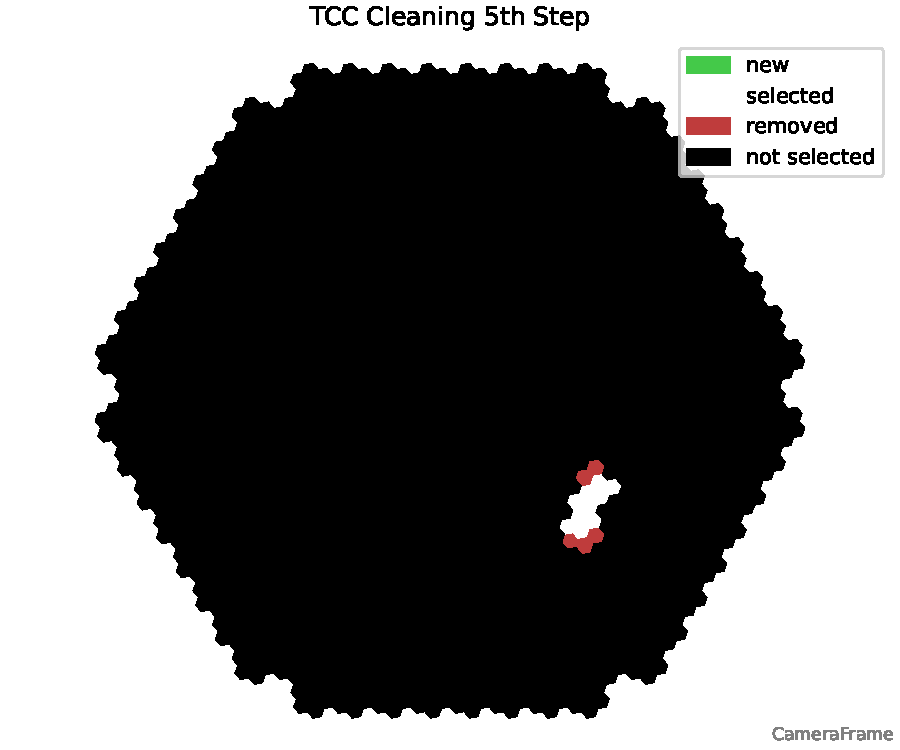
\includegraphics[width=\textwidth]{plots/cleaner_steps/tcc_5.pdf}
    % \end{subfigure}
    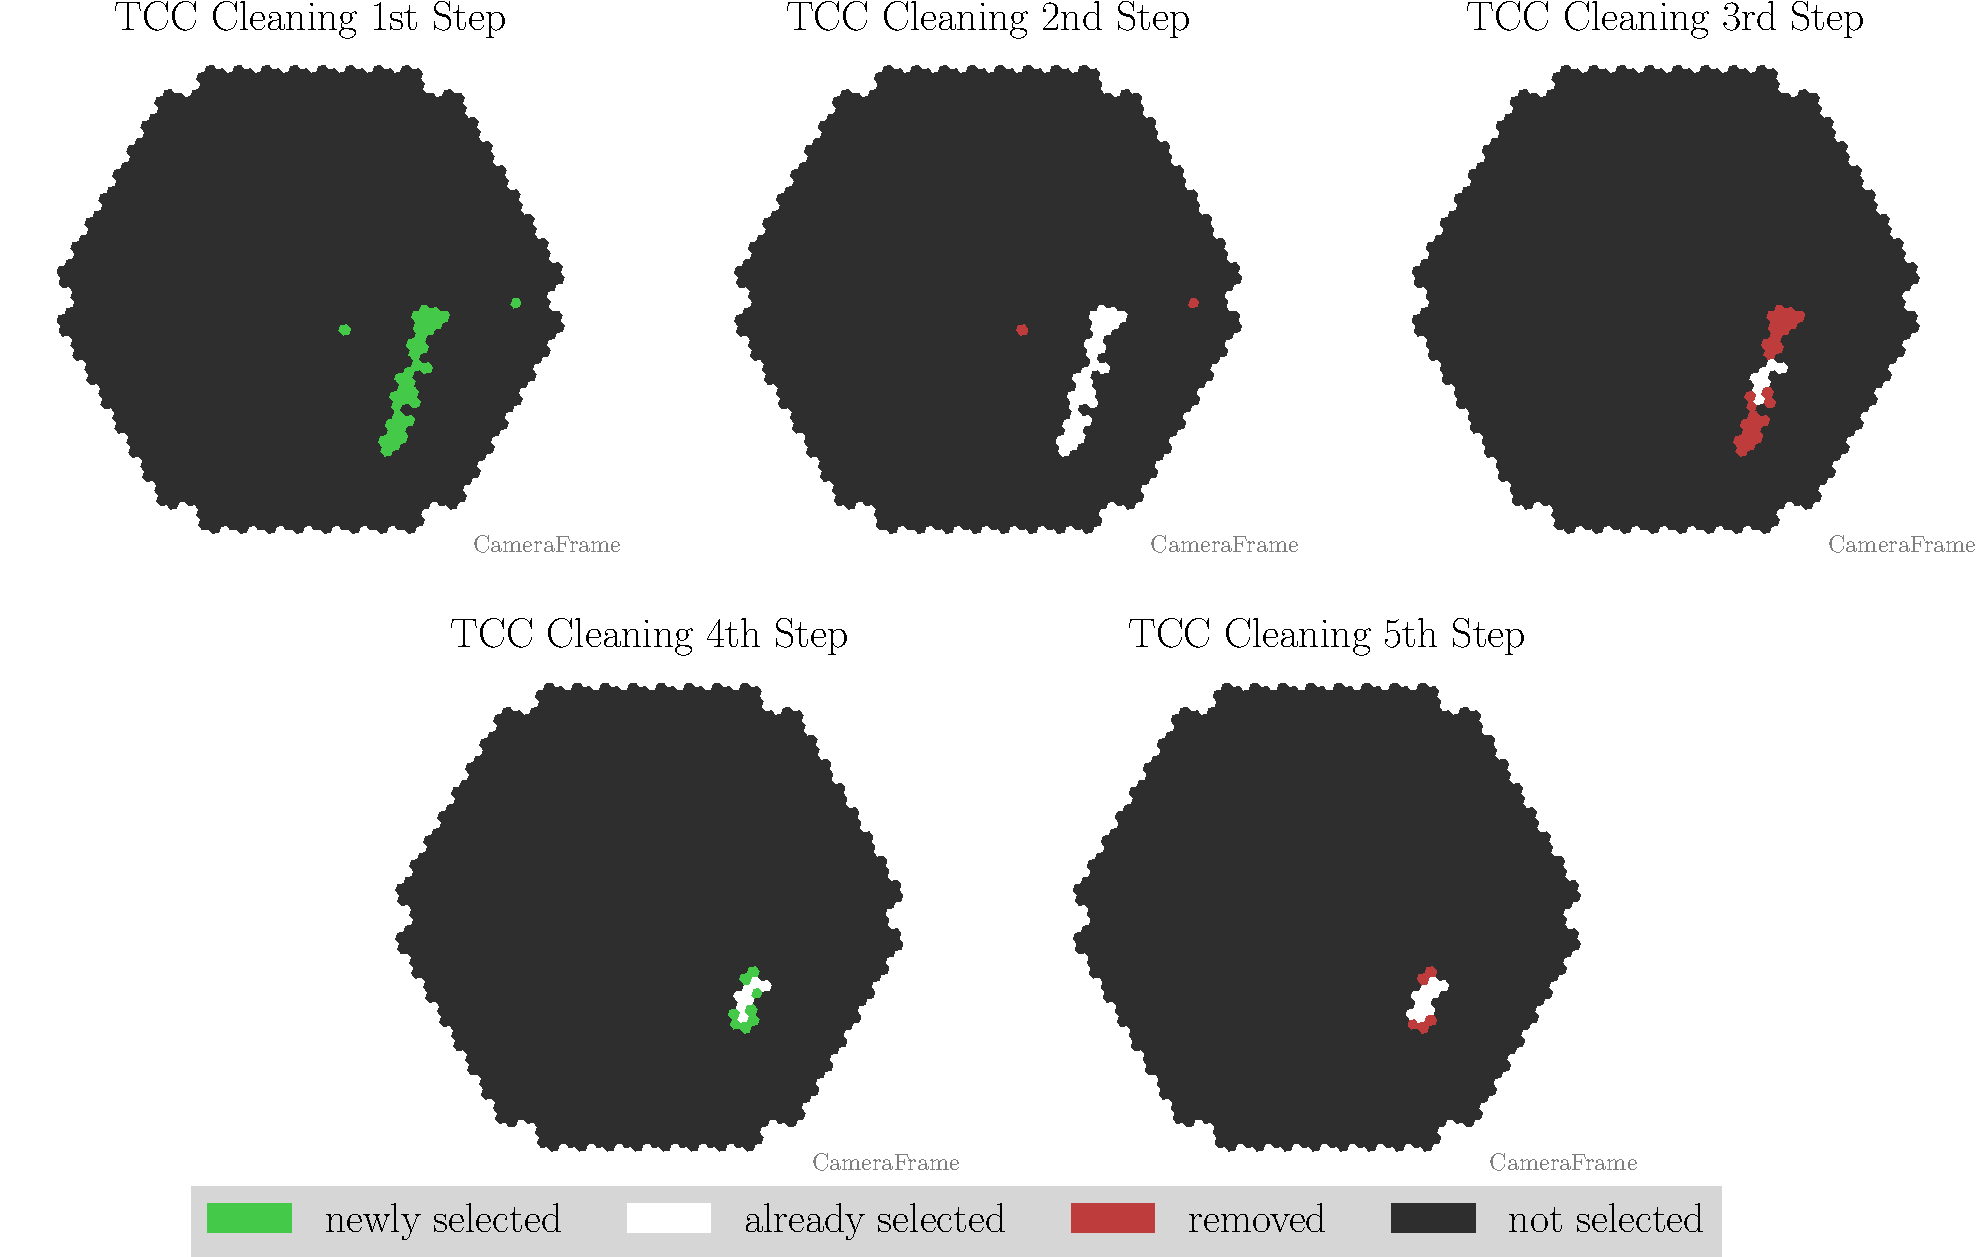
\includegraphics[height=8cm]{plots/cleaner_steps/tcc.pdf}
    \caption{Visualization of the \tcc{} algorithm for a \gls{mst} NectarCam image. The first step
    selects all pixels above the core threshold \(Q_c\). The second step removes all pixels that have less than
    \(N\) neighbors. The third step selects all pixels whose arrival times are within a given timeframe of the
    core time limit \(t_c\). The fourth step selects all pixels above the boundary threshold \(Q_b\).
    The fifth step removes all pixels with less than \(N\) neighbors that have arrived within a given timeframe
    of the boundary time limit \(t_b\). Notice, that with the default values \tcc{} tends to select fewer pixels
    than the other algorithms.}%
    \label{fig:tcc_cleaning}
\end{figure}
\vspace{-0.5cm}

\section{Hyperparameters}%
\label{sec:hyperparameters}

The hyperparameters of each cleaning algorithm are set in a specific \texttt{configuration} file. There,
the user can set and change the parameters, shown in \autoref{tab:hyperparameters}. \tailcuts{}
and \mars{} can be set-up with only three parameters: the \texttt{picture\_threshold}, the
\texttt{boundary\_threshold} and \texttt{min\_number\_picture\_neighbors}. The time-based algorithms
have additional parameters: First of all a \texttt{time\_limit} for \fact{} and then a \texttt{time\_limit\_core} as
well as a \texttt{time\_limit\_boundary} for \tcc{}.
\begin{table}
    \centering
    \caption{The four cleaning algorithms and their hyperparameters. Being the most basic algorithms,
    \tailcuts{} and \mars{} have only three parameters, while the \fact{} and \tcc{} algorithms have
    one and two additional time-based parameters, respectively. This table shows the default values
    and, if the parameters have them, also their units, as they are implemented in the \ctapipe{}
    source code.}%
    \label{tab:hyperparameters}
    \rowcolors{0}{white!92!black}{}
    \adjustbox{varwidth=\linewidth,scale=0.9}{%
    \begin{tabular}{l l l}
        \hiderowcolors%
        \textbf{Cleaning Algorithm} & \textbf{Hyperparameter} & \textbf{Default Values} \\
        \showrowcolors%
        \tailcuts{} & \texttt{picture\_threshold}               & \qquad\(\SI{7}{\pe}\) \\
                    & \texttt{boundary\_threshold}              & \qquad\(\SI{5}{\pe}\) \\
                    & \texttt{min\_number\_picture\_neighbors}  & \qquad\(\num{0}\) \\
        \addlinespace[0.5em]
        \mars{}     & \texttt{picture\_threshold}               & \qquad\(\SI{7}{\pe}\) \\
                    & \texttt{boundary\_threshold}              & \qquad\(\SI{5}{\pe}\) \\
                    & \texttt{min\_number\_picture\_neighbors}  & \qquad\(\num{0}\) \\
        \addlinespace[0.5em]
        \fact{}     & \texttt{picture\_threshold}               & \qquad\(\SI{4}{\pe}\) \\
                    & \texttt{boundary\_threshold}              & \qquad\(\SI{2}{\pe}\) \\
                    & \texttt{time\_limit}                      & \qquad\(\SI{5}{\nano\second}\) \\
                    & \texttt{min\_number\_picture\_neighbors}  & \qquad\(\num{2}\) \\
        \addlinespace[0.5em]
        \tcc{}      & \texttt{picture\_threshold}               & \qquad\(\SI{7}{\pe}\) \\
                    & \texttt{boundary\_threshold}              & \qquad\(\SI{5}{\pe}\) \\
                    & \texttt{time\_limit\_core}                & \qquad\(\SI{4.5}{\nano\second}\) \\
                    & \texttt{time\_limit\_boundary}            & \qquad\(\SI{1.5}{\nano\second}\) \\
                    & \texttt{min\_number\_picture\_neighbors}  & \qquad\(\num{1}\) \\
  \end{tabular}}
\end{table}

The full configuration files for the default settings of each cleaning algorithm are listed in
\hyperref[ap:config_files]{appendix~\ref{ap:config_files}}. There, the configuration files for the allowed telescopes
as described in \autoref{sec:pipeline} are shown, too.

To find the optimal hyperparameters, I utilized \sklearn{}~\cite{scikit-learn} for a grid search. This
allows one to manually set subsets of hyperparameters and search for the best combination of these.
\autoref{tab:hyperparameters_gridsearch} in \hyperref[ap:hyperparameters]{appendix~\ref{ap:hyperparameters}} shows
the subsets of hyperparameters used in this work.

I used noise quantiles, \ie the percentage of all \textit{noise} pixels that are not part of the true signal,
to determine the core threshold \(Q_c\). This would mean that \eg \(\SI{99.99}{\percent}\)
of the noise pixels would fall under a threshold of \(\SI{9.50}{\pe}\) for the data used in this work. The quantiles are calculated directly from the images by
discriminating the noise pixels from the image with the help of the true image. This approach has the
advantage that the resulting thresholds are more precisely optimized\footnote{As opposed to setting the thresholds by hand, \eg \numrange{4}{10} in \num{0.5} increments.}.
Since the boundary thresholds are calculated as a quotient of \(Q_c\), this benefits here as well.
The quantiles used in this work are shown in \autoref{fig:quantiles}.
\begin{figure}
    \centering
    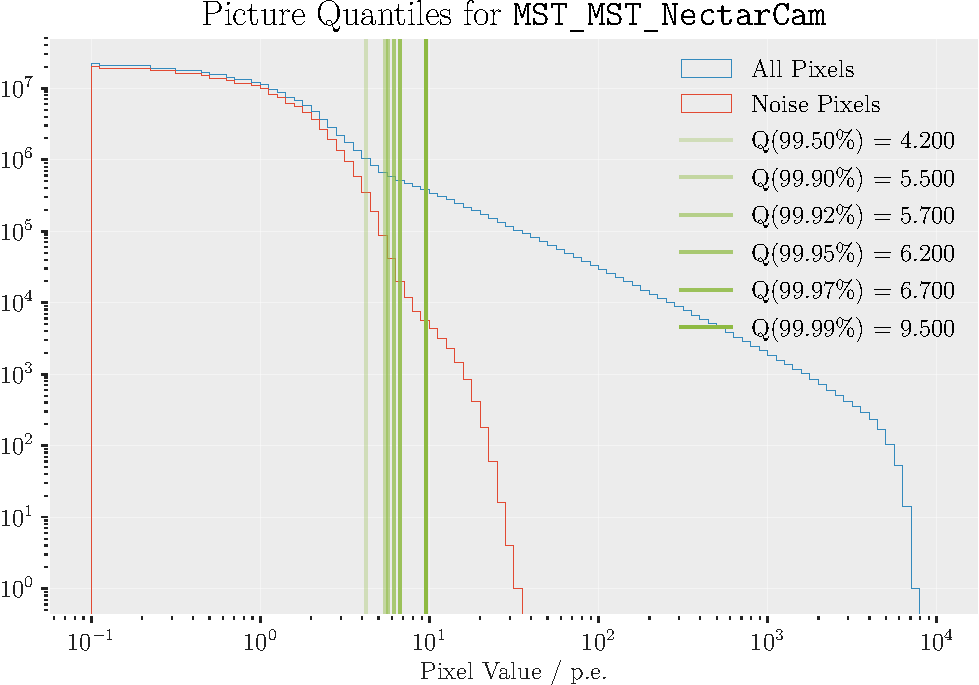
\includegraphics[width=\textwidth]{build/quantiles_plot.pdf}
    \caption{Picture noise quantiles for a \gls{mst} NectarCam dataset. The quantiles are calculated
    as the percentage of noise pixels in the image. The resulting threshold can then be used as a
    candidate for the core threshold \(Q_c\) in a grid search.}%
    % This method is more precise than selecting
    % the thresholds by hand, as they are calculated directly from the image.}
    \label{fig:quantiles}
    \vspace{-0.5cm}
\end{figure}
% To find the optimal hyperparameters, I used the \texttt{ParameterGrid} class from the
% \texttt{sklearn.model\_selection} module in \sklearn{}~\cite{scikit-learn}. The \texttt{ParameterGrid} class is useful to create a
% dictionary of all possible combinations of a list of given parameters. These combinations are then
% written to a config file and processed with \ctapipe{}. The output is hundreds of datasets equal to
% the number of combinations of the given parameters, each with a different setting for the cleaning
% performed on the data. The listing below shows the parameters fed into the \texttt{ParameterGrid}:
% % \enlargethispage{1\baselineskip}
% \begin{mdframed}[backgroundcolor=white!20!black,leftmargin=0cm,rightmargin=0cm, skipabove=0pt, innerleftmargin=0,innerrightmargin=0,]
%     \adjustbox{varwidth=\linewidth,scale=0.7}{%
%     \begin{pythonlst}
%         common_params = {
%             "picture_quantiles": (0.995, 0.999, 0.9992, 0.9995, 0.9997, 0.9999),
%             "boundary_threshold_ratio": (1/4, 1/3, 1/2, 2/3, 3/4),
%             "min_number_picture_neighbors": (1, 2, 3, 4, 5)
%         }
%         fact_params = {
%             "time_limit": (1.0, 2.0, 4.0, 5.0, 6.0, 10.0, 12.0)
%         }
%         tcc_params = {
%             "time_limit_core": (9.0, 12.0, 15.0, 18.0, 20.0),
%             "time_limit_boundary" = (4.5, 9.0, 12.0, 15.0)
%         }
%     \end{pythonlst}}
% \end{mdframed}

% The name \texttt{common\_params} is used here to refer to the dictionary of parameters that are common
% to all cleaning algorithms, while \texttt{fact\_params} and \texttt{tcc\_params} denote the additional
% hyperparameters exclusive to \fact{} and \tcc{}. The \texttt{picture\_quantiles} parameter determines
% how many percent of all pixels will be below the \texttt{picture\_threshold}. This is especially useful,
% as this results in a more precise value for the threshold\footnote{As opposed to setting the thresholds by hand, \eg{} \numrange{4}{10} in \num{0.5} increments}.
% The \texttt{boundary\_threshold\_ratio} sets
% the ratio of the \texttt{boundary\_threshold} \wrt the \texttt{picture\_threshold}. The other parameters,
% \texttt{min\_number\_picture\_neighbors} and the time limits are the same as explained before and are,
% therefore, absolute values.

The grid search results in \(\num{150}\) parameter combinations for \tailcuts{} and \mars{} each,
as well as another \(\num{1050}\) combinations for \fact{} and further \(\num{3000}\) combinations for \tcc{}.
Since it is impossible to find the optimal settings just by looking at the
cleaned images of the datasets, a combined metric is necessary to evaluate each cleaner's performance
for the parameter combinations.

In this work, I chose to first look at the efficiency
\begin{equation}\label{eq:efficiency}
    \eff =  \frac{n_{\mathrm{reco}}}{n_{\mathrm{total}}},
\end{equation}
where \(n_{\mathrm{total}}\) is the total number of events in the dataset and \(n_{\mathrm{reco}}\)
the number of reconstructed events. The latter depends on the cleaning, as only a successfully cleaned
event can be parametrized and therefore reconstructed. By first binning the efficiency per energy and then
taking the sum over all energy bins, one can sort the datasets by setting upper and lower bounds for the efficiency.
The intervals' lengths were chosen as \(\num{0.05}\), \ie \(\SI{5}{\percent}\), resulting in a total
of \(\num{20}\) intervals between \(\SI{0}{\percent}\) and \(\SI{100}{\percent}\).

For each interval, the mean angular resolution is calculated by determining the
\(\SI{68}{\percent}\) containment of the angular distance distribution, \ie the angular distance
between the reconstructed origin and the true origin of the shower.
% This angular distance, or separation, is calculated with the \texttt{astropy.coordinates.angular\_separation} function from \astropy{}~\cite{astropy1, astropy2}.
The dataset with the lowest mean angular resolution is the best performing for each interval.
If more low-energy events are reconstructed, not only will the efficiency be higher, but also the angular resolution,
as those events are more likely to include pixels that are part of the \gls{nsb} and also include fewer signal pixels
than a high-energy event.
% Not all events will ever be properly reconstructed for any parameter combination, so there won't be
% a mean angular resolution for all intervals, but only a subset.
% Also, the mean angular resolution may be higher when more events were reconstructed.
As a result, a trade-off between efficiency and angular resolution is necessary.

For the performance analysis of the algorithms, I calculated metrics such as, but not limited to, the \gls{tpr} or recall,
the \gls{fpr} or fall-out and the \gls{tnr} or specificity. A list of all used metrics can be seen in \autoref{tab:metrics}
in \hyperref[ap:metrics]{appendix~\ref{ap:metrics}}.